** REMEMBER TEXT! **

\section{Pre-processing}

The data is pre-processed in MatLab, where pain maps are superimposed onto the knee regions. When importing pictures into MatLab a matrix is created. The pain map is converted into a matrix consisting of zeroes and ones, where the pain is symbolised with ones.  
Since the knee regions shown in figure \ref{fig:atlas} is a picture with three layers consisting of RGB colors, the picture is divided into three matrices, that enables the regions to be labeled in a new matrix. The two matrices, pain map and the labeled knee regions, are superimposed, which results in a matrix with only zeroes and the regions with pain. 
An illustration of the pre-processing step is shown in figure \ref{fig:preproc}.

\begin{figure} [H]
\centering
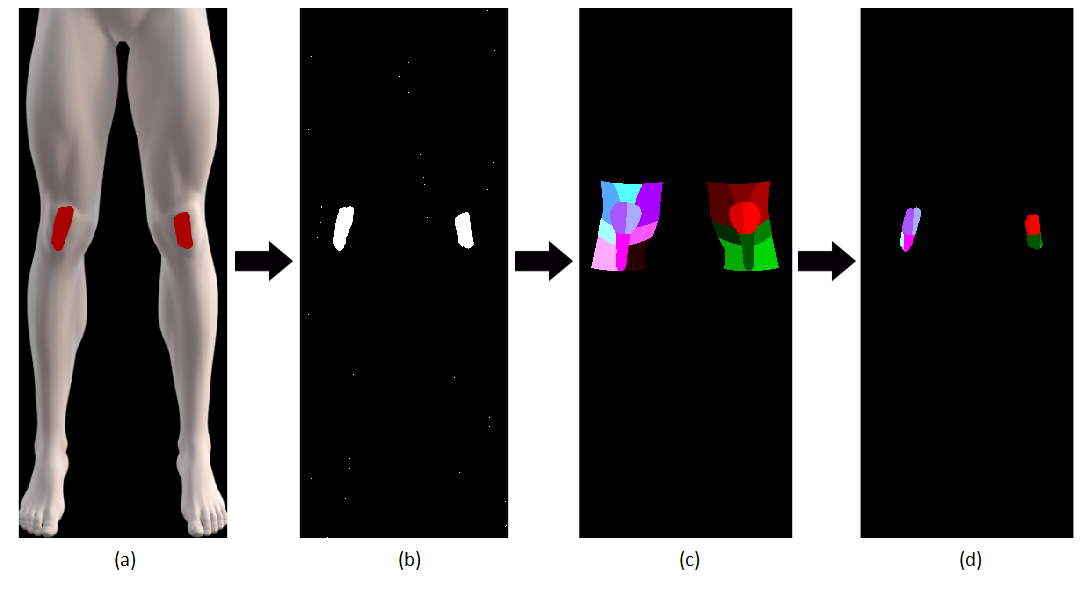
\includegraphics[width=1\textwidth]{figures/preprocessing}
\caption{The figure illustrates the pre-processing step. (a) is the raw pain map, (b) is the matrix of pain, (c) is the pain regions and (d) is the active pain regions.}
\label{fig:preproc}
\end{figure}

\noindent
\autoref{fig:preproc}(a) is the raw pain map, and (b) is the pain transferred to a matrix consisting of zeroes and ones, which is shown as black and white, where white areas are ones in the matrix. In figure \ref{fig:preproc}(b) is there white spots, these spots is removed with a filter. \autoref{fig:preproc}(c) illustrates the pain regions, each region is colored in relate to the set label, which permits the comparison of the pain and regions, that is shown in figure \ref{fig:preproc}(d).  
